% --- [ Back-end Components ] --------------------------------------------------

\subsection{Back-end Components}
\label{sec:design_back-end_components}

The back-end module translates structured LLVM IR into a target high-level programming language, using two distinct stages. Firstly, the code generation stage translates LLVM IR into unpolished Go code by converting the individual instructions into equivalent Go statements and creating high-level control flow primitives for the various basic blocks, using the information of the structured CFGs (see section \ref{sec:design_control_flow_analysis}). Secondly, the post-processing stage improves the quality of the unpolished Go code, through a series of source code transformations. The interaction between the middle-end, and the \texttt{ll2go} and \texttt{go-post} tools of the back-end is illustrated in figure \ref{fig:back-end}.

\begin{figure}[htbp]
	\begin{center}
		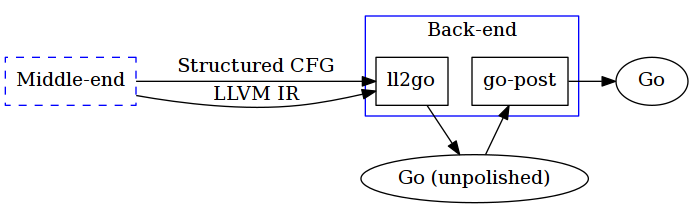
\includegraphics[width=0.8\textwidth]{inc/6_design/back-end.png}
		\caption{The back-end module decompiles structured LLVM IR into Go source code, using two components. The \texttt{ll2go} tool translates structured LLVM IR assembly into unpolished Go code, which is post-processed by the \texttt{go-post} tool to improve the quality of the output.}
		\label{fig:back-end}
	\end{center}
\end{figure}

The clear distinction between the two back-end stages aligns with the design principle of separation of concern. The code generation stage may focus on converting LLVM IR into equivalent Go code, without having to worry about the quality of the produced code. Similarly, the post-processing stage may focus on simplifying the Go code and make it more idiomatic, without any knowledge of the underlying LLVM IR. This enables the post-processing component to be reused as-is by other projects to improve the quality of Go code.

A tighter integration between the two stages could potentially produce a higher quality output, but there are no known issues preventing the decoupled stages from producing output of equivalent quality.

The decompilation pipeline aims to keep the back-end module as simple as possible, by delegating general decompilation tasks (e.g. control flow analysis, data flow analysis) to the middle-end module. This reduces the efforts required to implement additional back-ends, which add support for new target programming languages (e.g. Python).

% --- [ Subsubsections ] -------------------------------------------------------

% ~~~ [ Code Generation ] ~~~~~~~~~~~~~~~~~~~~~~~~~~~~~~~~~~~~~~~~~~~~~~~~~~~~~~

\subsubsection{Code Generation}
\label{sec:design_code_generation}

%    - Structured CFG -> Go ([ll2go](http://decomp.org/x/cmd/ll2go))
%       + Truthfully `ll2go` does not make direct use of `restructure` but rather the graph libraries.

foo

% Generates an abstract syntax tree (AST)

% ~~~ [ Post-processsing ] ~~~~~~~~~~~~~~~~~~~~~~~~~~~~~~~~~~~~~~~~~~~~~~~~~~~~~

\subsubsection{Post-processing}

%    - Unpolished Go -> Go ([go-post](http://decomp.org/x/cmd/go-post))

foo

The polishing is done by separate tools which fixes potential compilation issues and makes the code more idiomatic.

Currently the \texttt{go-post} replaces return-statements in the \texttt{main} function with calls to \texttt{os.Exit}, which is required since the \texttt{main} function has no return arguments in Go. Instead the Go runtime calls \texttt{os.Exit} with the status-code \texttt{0} once \texttt{main} returns to signal successful termination. This eliminates the need to always end the \texttt{main} function with a \texttt{return 0;} statement as is common practise in C. A future ambition is to make use of and possibly contribute to the \texttt{grind} tool which moves variable declarations closer to their usage, and thus improving readability of the code.

